\section{Introduction}
\vspace{-2em}

High-altitude ballooning has long served as an inexpensive flight platform for testing remote sensing instrumentation for Earth and space applications, communication systems, and other spaceflight hardware, offering quick turnaround and operational flexibility~\cite{HAB_Fundamentals}. The versatility of a high-altitude balloon flight provides a multidisciplinary platform for experiential learning, enabling students to design and execute a wide range of experiments shaped by both educational objectives and technical constraints. \par

%, as seen in Figure~\ref{Fig:HAB_Flight}

\begin{comment}
\begin{figure}[H]
    \centering
    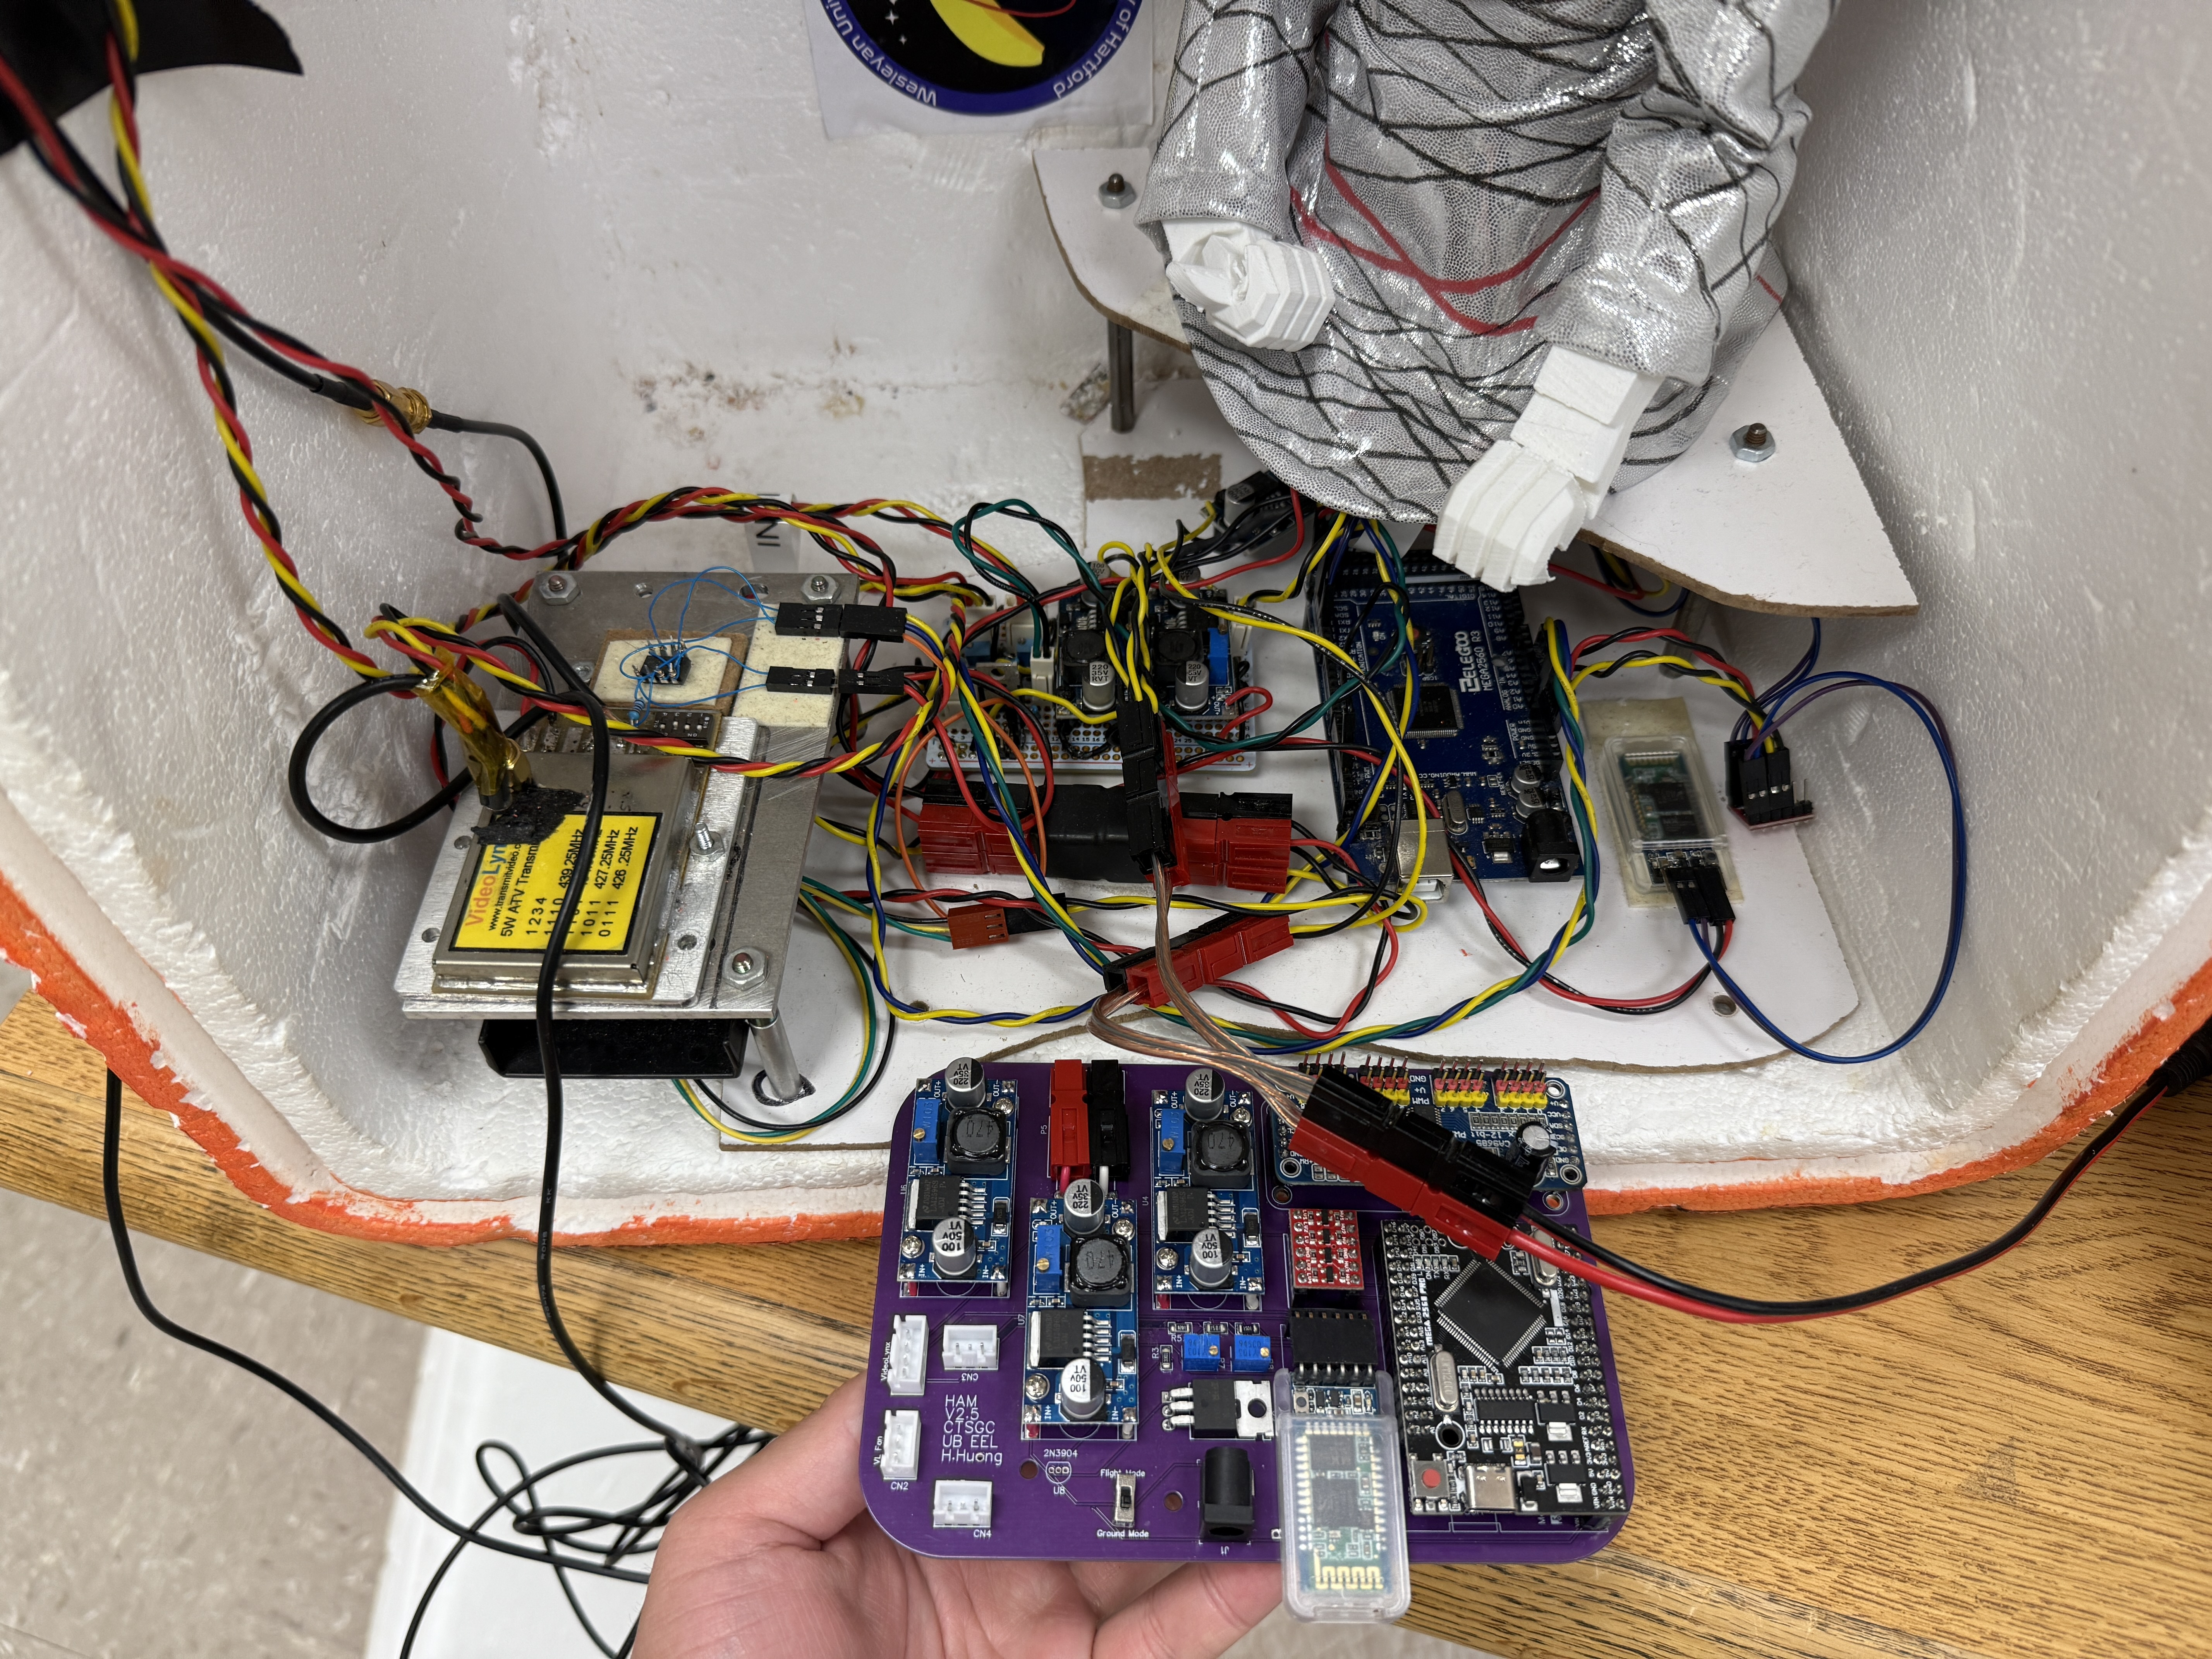
\includegraphics[width = 0.7\textwidth]{Figures/HAM_Wiring_Comparison.jpg}
    \caption{High Altitude Ballooning Flight}
    \label{Fig:HAB_Flight}
\end{figure}
\vspace{-2em}  % Reduce space after the figure
\end{comment}

HAM (an acronym for High Altitude Monkey) was developed by undergraduate students at the University of Bridgeport in 2015 as part of their fulfillment of the Bachelor of Science degree requirements in Electrical Engineering and Computer Science. The payload was named in homage to Ham, the first chimpanzee to travel into space aboard the Mercury-Redstone 2 mission in 1961, a historic milestone in human spaceflight~\cite{Burgess2014}. 

\begin{figure}[H]
    \centering
    \includegraphics[width = 0.6\textwidth]{Figures/HAM_Original_Flight.png}
    \caption{Still image from HAM’s maiden launch in November 2019}
    \label{Fig:HAB_2019_Flight}
\end{figure}
\vspace{-2em}  % Reduce space after the figure
Weighing just under 12 pounds, HAM completed its maiden flight in November 2019 over Bridgeport, Connecticut, where the payload was used to engage attendees at a local children's museum during a special outreach event. Figure~\ref{Fig:HAB_2019_Flight} shows HAM successfully establishing communication at an altitude of 500 feet, transmitting telemetry data and receiving movement commands in real time. The flight traveled approximately 14 miles east, reaching a peak altitude of 4,000 feet before landing on a beach in Milford, Connecticut. \par

In the 2024–2025 academic year, students in the Extreme Environments Laboratory aim to conduct a second flight using a redesigned model of HAM, incorporating nearly a decade of technological advancements. This study outlines the steps taken to improve HAM's 3D modeling and wiring, with the goal of enhancing the payload's efficiency and reducing its weight. It also explores potential design modifications and broader applications of HAM in future high-altitude ballooning missions.

\vspace{-2em}
\section{Structure and Subsystems}
\vspace{-2em}

This system is designed to utilize amateur radio frequencies for data transmission and is capable of operating at altitudes up to 10{,}000~feet (approximately 3~kilometers). The 2019 flight system consisted of two primary components: (1) an onboard telemetry and communications payload employing a TinyTrak4 module from Byonics~\cite{byonics_tinytrak4}, and (2) the main visual payload, shown in Figure~\ref{Fig:HAB_2015_Inside}, which transmitted black-and-white video signals over amateur radio frequencies. Data packets were transmitted and received using the Automatic Packet Reporting System (APRS), enabling real-time interpretation and display at the ground command center, as illustrated in Figure~\ref{Fig:HAB_2015_Command}. From this station, children were able to interact with HAM live during the mission. Commands sent from the ground were received by the telemetry payload and relayed to the visual payload via a local Bluetooth network using HC-05 modules. After executing the command, the telemetry system transmitted confirmation back to the ground, enabling the next command to be issued.

\begin{figure}[H]
    \centering
    \begin{subfigure}[t]{0.49\textwidth}
        \centering
        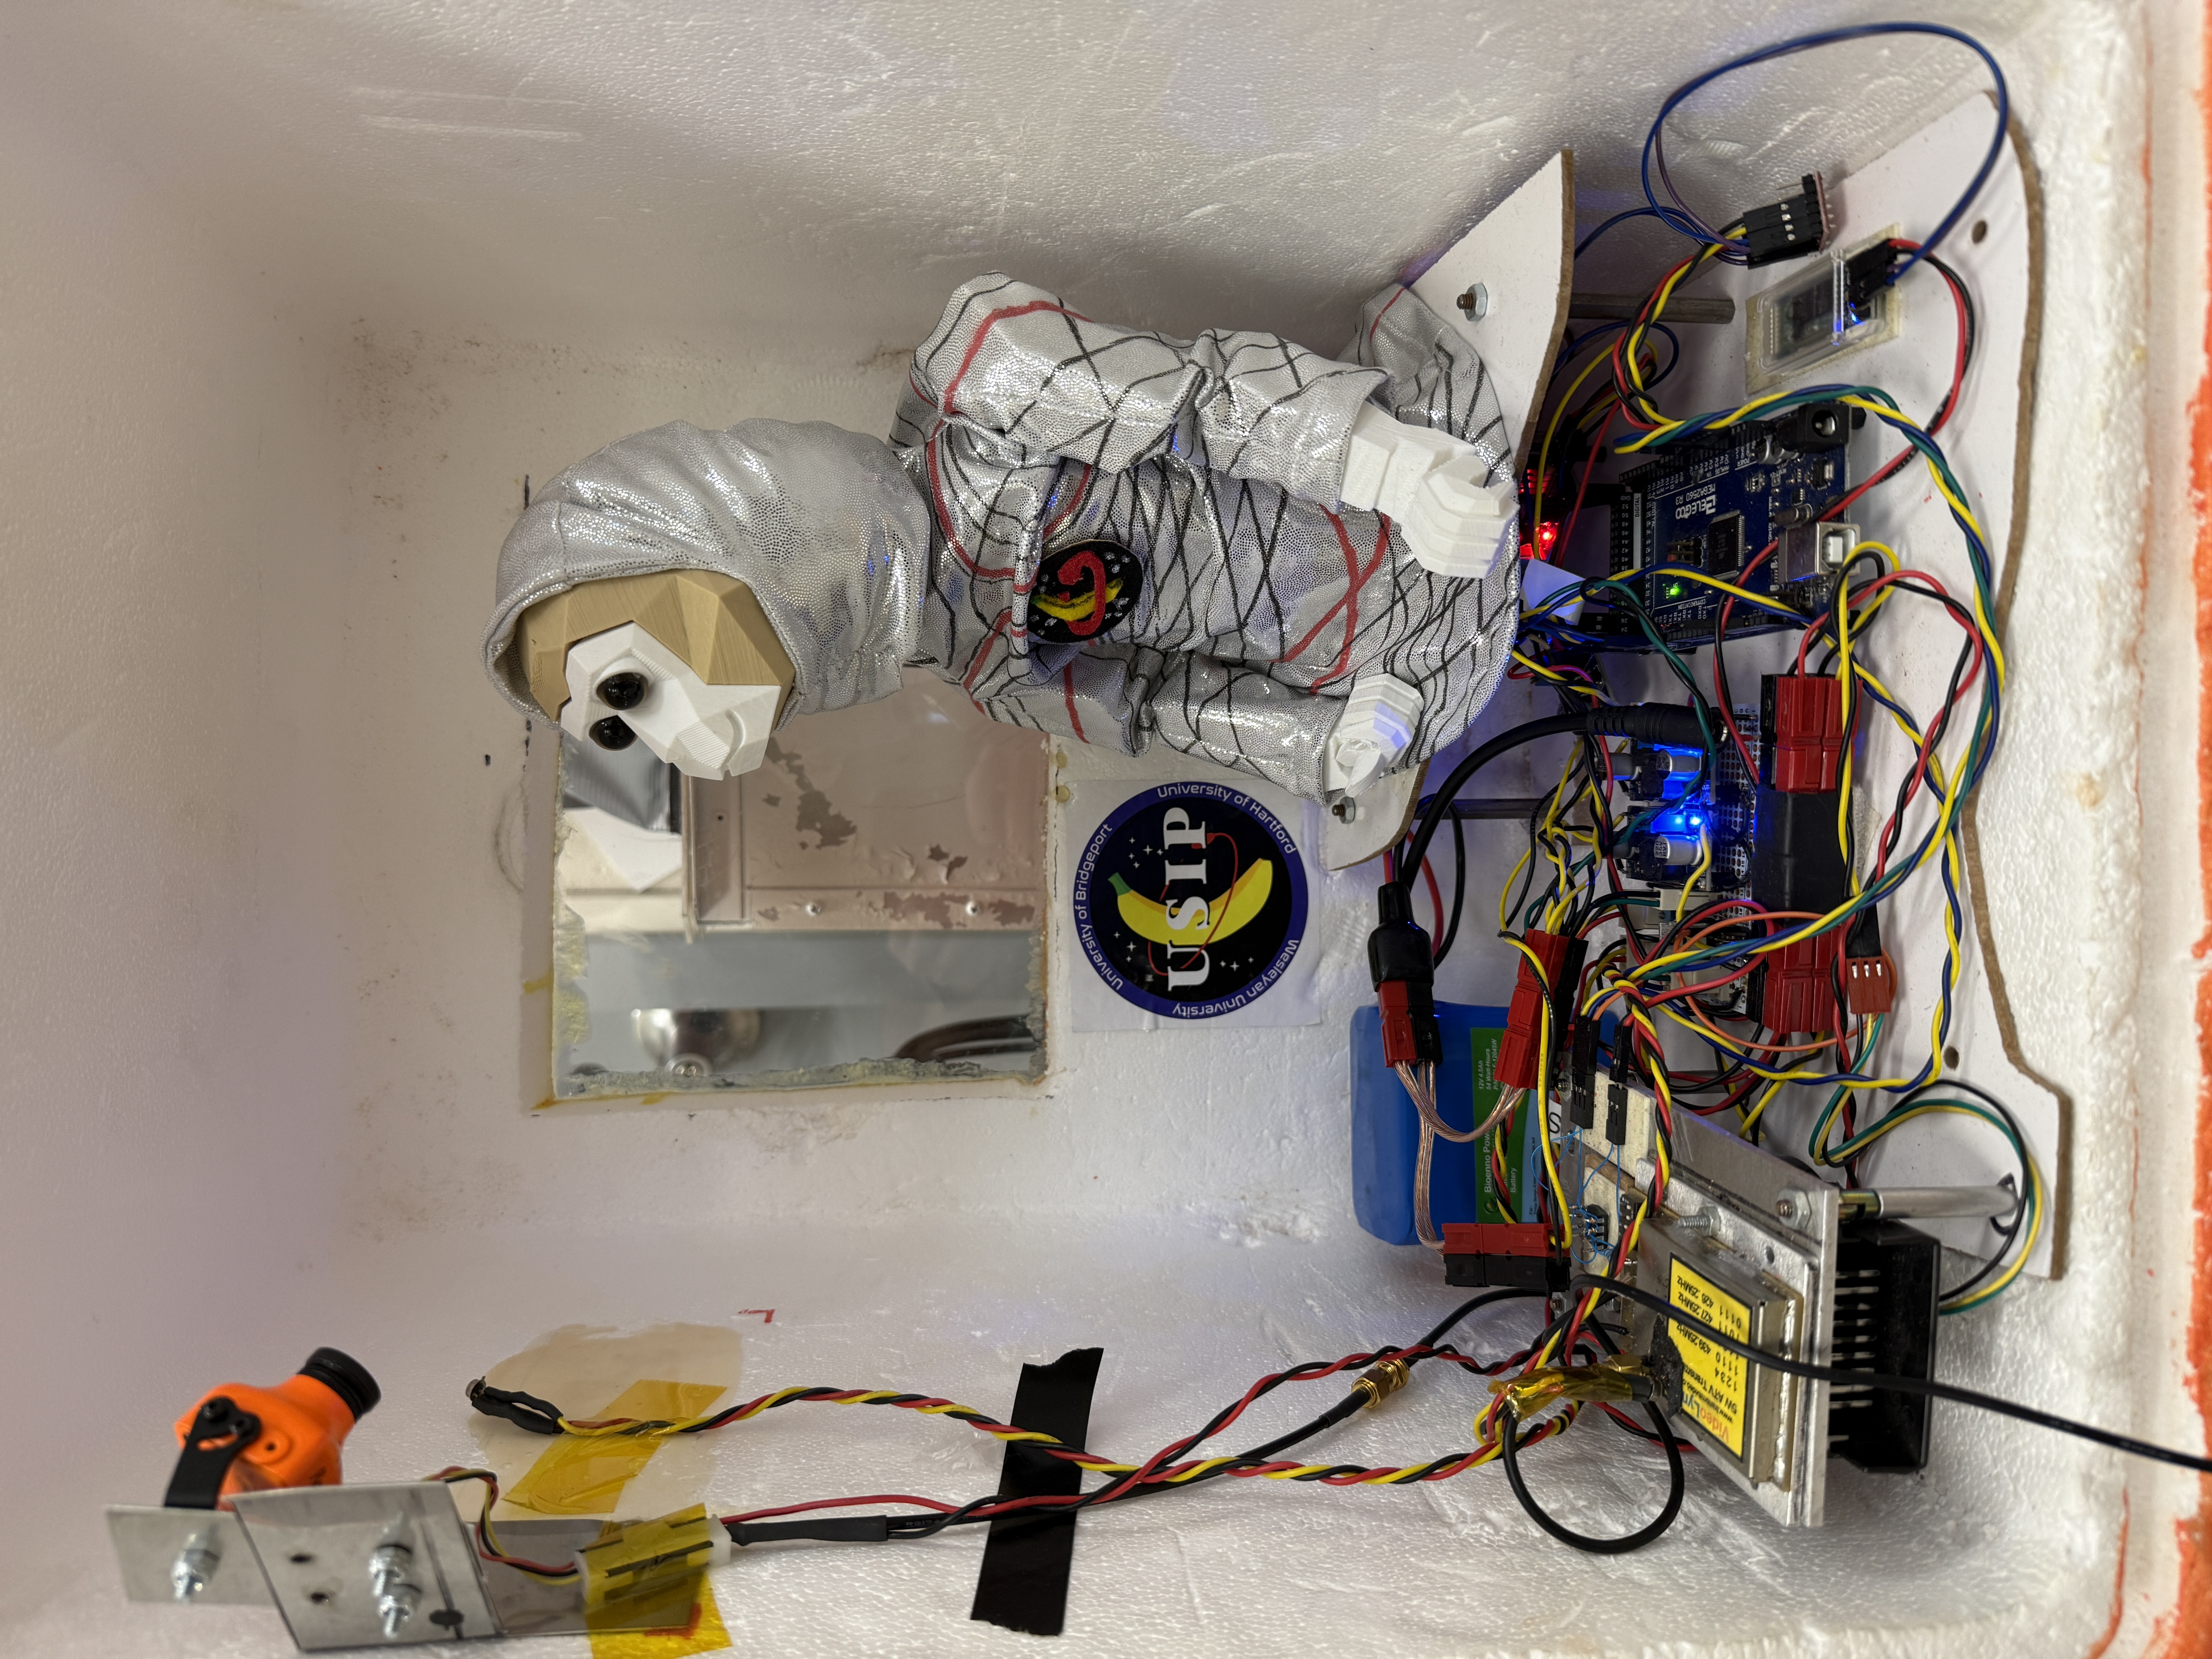
\includegraphics[width=\textwidth, angle=-90]{Figures/HAM_Original.JPG}
        \caption{Internal view of primary robotics payload}
        \label{Fig:HAB_2015_Inside}
    \end{subfigure}
    \hfill
    \begin{subfigure}[t]{0.49\textwidth}
        \centering
        \includegraphics[width=\textwidth, angle=-90]{Figures/Command_Processor.JPG}
        \caption{Command processing unit}
        \label{Fig:HAB_2015_Command}
    \end{subfigure}
    \caption{Overview of HAM's 2015 internal components and control systems configuration}
    \label{Fig:HAB_2015_Combined}
\end{figure}
\vspace{-2em}

The updated configuration will feature streamlined circuitry through printed circuit boards (PCBs), along with a reduction in overall payload weight. Additional upgrades include dual GPS tracking systems for improved accuracy and redundancy, an onboard venting system for precise control of ascent and descent, a cut-down mechanism for safe recovery, and a 360\degree{} camera to document HAM’s flight and enhance operational safety. \par

The research conducted in this project is highly novel within the field of high-altitude ballooning. Most flight systems rely on static payloads that primarily transmit data to the ground, without incorporating mechanical motion or interactive components. HAM distinguishes itself as a unique innovation by integrating constant bidirectional communication, moving mechanisms, and real-time telemetry, all streamed to the ground via live video feed. \par